\documentclass[aspectratio=169]{beamer}
\usetheme{Madrid}
\usecolortheme{default}
\usepackage{booktabs}
\usepackage{graphicx}
\usepackage{xcolor}
\usepackage{amsmath}

\title{Landslide Identification Using ML}
\subtitle{Lifecycle 2: Optimization \& Ensemble Strategies}
\author{M.Tech Project}
\date{2026-03-18}

\begin{document}

% ---- Slide 1: Title ----
\begin{frame}
    \titlepage
\end{frame}

% ---- Slide 2: LC1 Recap ----
\begin{frame}{Recap: Lifecycle 1 Outcomes}
    \textbf{What we built:}
    \begin{itemize}
        \item Dual-phase pipeline: CNN classification + HMM temporal forecasting
        \item Tested AlexNet (scratch \& pretrained) and EfficientNet-B3
        \item Best result: EfficientNet-B3 --- 79.97\% accuracy, 70.21\% F1, 88.93\% AUC
    \end{itemize}

    \vspace{0.4cm}
    \textbf{Gaps identified:}
    \begin{enumerate}
        \item Model is \textbf{overconfident} --- says 95\% when only 75\% accurate
        \item \textbf{Single model} has systematic blind spots (94 false positives)
        \item HMM too \textbf{simplistic} --- only 7 observation symbols
        \item Decision threshold (50\%) is \textbf{arbitrary}
    \end{enumerate}
\end{frame}

% ---- Slide 3: LC2 Objectives ----
\begin{frame}{Lifecycle 2 Objectives}
    \begin{enumerate}
        \item \textbf{Calibrate confidence scores} --- temperature scaling
        \item \textbf{Combine models} --- ensemble to cancel individual errors
        \item \textbf{Upgrade HMM} --- add trigger mechanisms (42 symbols)
        \item \textbf{Introduce Vision Transformer} --- global spatial features
        \item \textbf{Optimize threshold} --- data-driven, not arbitrary
    \end{enumerate}
\end{frame}

% ---- Slide 4: Result 3 — Temperature Scaling ----
\begin{frame}{Result 3: Temperature Scaling + HMM Upgrade}
    \textbf{Temperature Scaling:}
    \begin{itemize}
        \item Learned temperature $T = 1.1511$ on validation set
        \item Divides logits by $T$ before softmax: $\hat{q}_i = \frac{\exp(z_i/T)}{\sum_j \exp(z_j/T)}$
        \item Does NOT change predictions --- fixes confidence scores only
        \item Now: 70\% confidence $\approx$ 70\% true accuracy
    \end{itemize}

    \vspace{0.3cm}
    \textbf{HMM Upgrades:}
    \begin{itemize}
        \item Hidden states: 4 $\to$ \textbf{8} (finer regimes)
        \item Observation symbols: 7 $\to$ \textbf{42} (type $\times$ trigger)
        \item Example: distinguishes ``monsoon debris flow'' from ``earthquake rockfall''
    \end{itemize}
\end{frame}

% ---- Slide 5: Result 4 — Ensemble ----
\begin{frame}{Result 4: Ensemble + Optimal Threshold}
    \textbf{Ensemble Strategy:}
    \[
    P_{\text{ensemble}} = 0.6 \times \text{softmax}(\mathbf{z}_{\text{EfficientNet}} / T) + 0.4 \times \text{softmax}(\mathbf{z}_{\text{AlexNet}})
    \]

    \begin{itemize}
        \item EfficientNet: higher recall (catches more landslides)
        \item AlexNet: relatively higher precision (fewer false alarms)
        \item Combined: errors cancel out $\to$ all 5 metrics improve
    \end{itemize}

    \vspace{0.3cm}
    \textbf{Optimal Threshold:} 50\% $\to$ \textbf{46.7\%} (from PR curve analysis)

    \vspace{0.2cm}
    \begin{table}
        \centering
        \small
        \begin{tabular}{lccccc}
            \toprule
            & Acc & Prec & Rec & F1 & AUC \\
            \midrule
            r2 (single) & 79.97 & 63.71 & 78.20 & 70.21 & 88.93 \\
            \textbf{r4 (ensemble)} & \textbf{82.40} & \textbf{68.03} & \textbf{78.67} & \textbf{72.97} & \textbf{89.83} \\
            \bottomrule
        \end{tabular}
    \end{table}
\end{frame}

% ---- Slide 6: Result 5 — ViT Ensemble ----
\begin{frame}{Result 5: CNN + Transformer Hybrid Ensemble}
    \textbf{Why replace AlexNet with ViT-B/16?}
    \begin{itemize}
        \item Two CNNs share the same blind spot: only see \textit{local} textures
        \item ViT uses self-attention $\to$ sees \textit{global} spatial relationships
        \item CNN + Transformer = genuinely \textbf{diverse} ensemble
    \end{itemize}

    \vspace{0.3cm}
    \[
    P = 0.6 \times \text{EfficientNet-B3} + 0.4 \times \text{ViT-B/16}
    \]

    \begin{table}
        \centering
        \small
        \begin{tabular}{lccccc}
            \toprule
            & Acc & Prec & Rec & F1 & AUC \\
            \midrule
            r4 (CNN+CNN) & 82.40 & 68.03 & 78.67 & 72.97 & 89.83 \\
            \textbf{r5 (CNN+ViT)} & \textbf{84.55} & \textbf{71.50} & \textbf{81.04} & \textbf{75.98} & \textbf{91.50} \\
            \bottomrule
        \end{tabular}
    \end{table}

    \textbf{Biggest single improvement in the project:} F1 +3.01\%, AUC +1.67\%
\end{frame}

% ---- Slide 7: Evaluation Output ----
\begin{frame}{Evaluation Output: Confusion Matrix \& ROC Curve}
    \begin{columns}
        \begin{column}{0.5\textwidth}
            \centering
            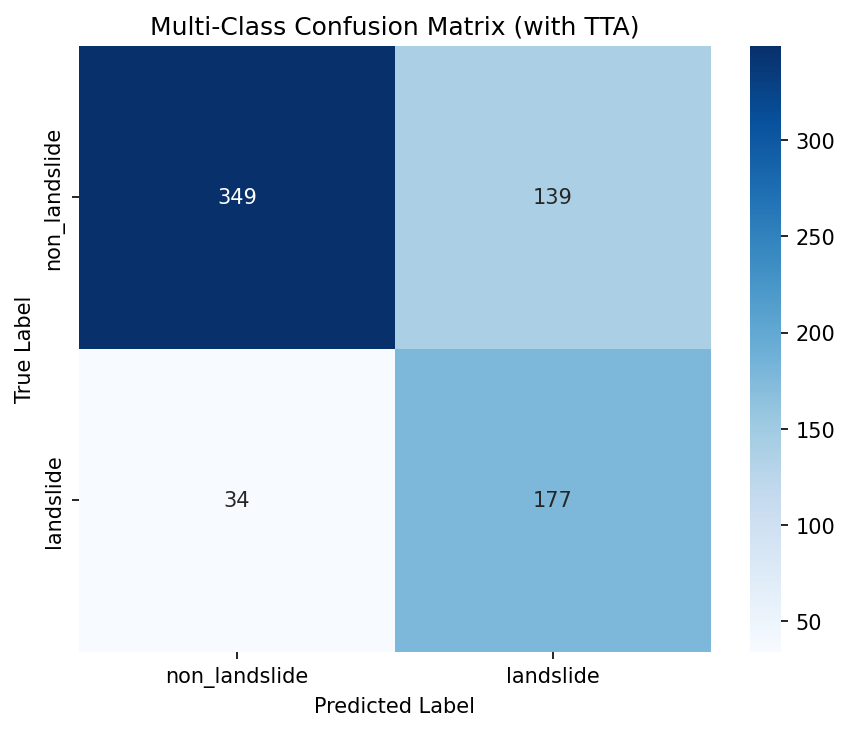
\includegraphics[width=0.95\textwidth]{project/plots/confusion_matrix.png}\\[0.1cm]
            \small After ensemble: fewer false negatives (missed landslides reduced)
        \end{column}
        \begin{column}{0.5\textwidth}
            \centering
            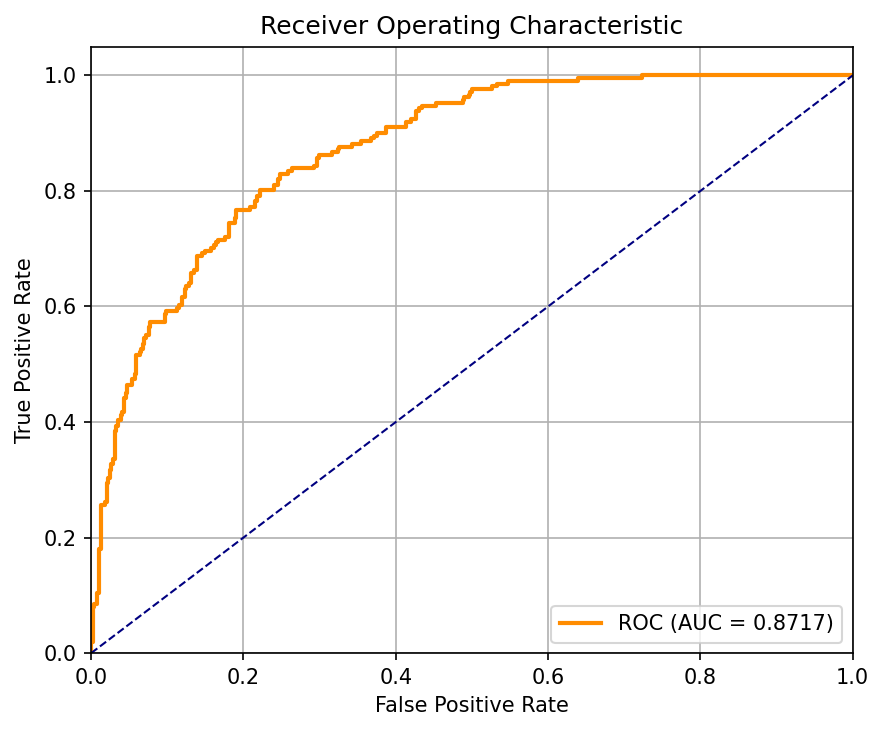
\includegraphics[width=0.95\textwidth]{project/plots/roc_curve.png}\\[0.1cm]
            \small AUC improved from 88.93\% (r2) to 91.50\% (r5)
        \end{column}
    \end{columns}
\end{frame}

% ---- Slide 8: Pipeline Demo ----
\begin{frame}[fragile]{Pipeline Output: Ensemble Prediction}
    \textbf{What happens during ensemble prediction:}
    \begin{enumerate}
        \item Same image goes through \textbf{both} EfficientNet-B3 and ViT-B/16
        \item EfficientNet outputs: [0.30, 0.70] (70\% landslide)
        \item ViT outputs: [0.45, 0.55] (55\% landslide)
        \item Weighted average: $0.6 \times 0.70 + 0.4 \times 0.55 = 0.64$ (64\% landslide)
        \item 64\% $\geq$ 46.7\% threshold $\to$ \textbf{LANDSLIDE DETECTED}
    \end{enumerate}

    \vspace{0.3cm}
    \textbf{Terminal output:}
    \begin{verbatim}
Phase 1 - LANDSLIDE (confidence: 64.0%)
Phase 2 - Type: Debris Flow
          Occurrence probability: 30.0%
          Peak risk month: July
    \end{verbatim}

    \small Even when individual models are uncertain, the ensemble can make a confident decision.
\end{frame}

% ---- Slide 9: Cumulative Comparison ----
\begin{frame}{Cumulative Progress: r0 $\to$ r5}
    \begin{table}
        \centering
        \renewcommand{\arraystretch}{1.2}
        \small
        \begin{tabular}{llccccc}
            \toprule
            \textbf{Result} & \textbf{Architecture} & \textbf{Acc} & \textbf{Prec} & \textbf{Rec} & \textbf{F1} & \textbf{AUC} \\
            \midrule
            r0 & AlexNet (scratch) & 78.54 & 62.06 & 74.41 & 67.67 & 85.53 \\
            r1 & AlexNet (pretrained) & 80.11 & 66.67 & 67.30 & 66.98 & 85.73 \\
            r2 & EfficientNet-B3 & 79.97 & 63.71 & 78.20 & 70.21 & 88.93 \\
            r3 & + Temp Scaling & 79.97 & 63.71 & 78.20 & 70.21 & 88.93 \\
            r4 & + Ensemble & 82.40 & 68.03 & 78.67 & 72.97 & 89.83 \\
            \textbf{r5} & \textbf{+ ViT Ensemble} & \textbf{84.55} & \textbf{71.50} & \textbf{81.04} & \textbf{75.98} & \textbf{91.50} \\
            \bottomrule
        \end{tabular}
    \end{table}

    \vspace{0.3cm}
    \textbf{Total improvement over baseline:}
    Accuracy +6.01\%, F1 +8.31\%, AUC +5.97\%
\end{frame}

% ---- Slide 8: Key Findings ----
\begin{frame}{Key Findings from Lifecycle 2}
    \begin{enumerate}
        \item \textbf{Architectural diversity $>$ model count}
            \begin{itemize}
                \item CNN + Transformer much better than CNN + CNN
                \item Different inductive biases produce complementary errors
            \end{itemize}
        \item \textbf{Calibration enables reliable thresholding}
            \begin{itemize}
                \item Temperature scaling makes confidence scores operationally meaningful
            \end{itemize}
        \item \textbf{HMM with triggers produces better forecasts}
            \begin{itemize}
                \item Type $\times$ trigger (42 symbols) captures environmental context
            \end{itemize}
        \item \textbf{Ensemble is a zero-cost improvement}
            \begin{itemize}
                \item Combines existing checkpoints --- no retraining needed
            \end{itemize}
    \end{enumerate}
\end{frame}

% ---- Slide 9: Remaining Gaps ----
\begin{frame}{Remaining Gaps to Address}
    \begin{enumerate}
        \item \textbf{Class imbalance} (72\% non-landslide vs 28\% landslide)
            \begin{itemize}
                \item Cross-Entropy treats all samples equally $\to$ biased toward majority
                \item Still 40 false negatives (missed landslides)
            \end{itemize}

        \item \textbf{Single-pass inference fragility}
            \begin{itemize}
                \item Same landslide, different orientation $\to$ different prediction
                \item Some false negatives had confidence 44--46\% (just below threshold)
            \end{itemize}

        \item \textbf{Black-box predictions}
            \begin{itemize}
                \item Model outputs a number, but \textit{why}?
                \item Disaster teams can't trust what they can't verify
                \item Explainability required for safety-critical deployment
            \end{itemize}
    \end{enumerate}
\end{frame}

% ---- Slide 10: LC3 Preview ----
\begin{frame}{Lifecycle 3 Preview: Advanced Techniques \& Deployment}
    \textbf{Three improvements targeting three pipeline stages:}

    \vspace{0.3cm}
    \begin{enumerate}
        \item \textbf{Focal Loss} (Training)
            \begin{itemize}
                \item Down-weights easy examples, focuses on hard borderline cases
                \item Directly addresses class imbalance $\to$ expected +2--4\% recall
            \end{itemize}

        \item \textbf{Test-Time Augmentation} (Inference)
            \begin{itemize}
                \item 5 augmented views per image, average predictions
                \item Rescues borderline cases $\to$ expected +1--3\% recall
            \end{itemize}

        \item \textbf{Grad-CAM} (Explainability)
            \begin{itemize}
                \item Heatmaps showing \textit{where} the model looks
                \item Verify predictions are based on geological features, not artifacts
                \item Critical for disaster response trust
            \end{itemize}
    \end{enumerate}

    \vspace{0.2cm}
    \centering
    \textbf{Train better $\to$ Predict better $\to$ Explain better}
\end{frame}

% ---- Slide 13: Thank You ----
\begin{frame}{}
    \centering
    \vspace{2cm}
    {\Large \textbf{Thank You}}

    \vspace{1cm}
    Questions \& Discussion
\end{frame}

\end{document}
